
%(BEGIN_QUESTION)
% Copyright 2010, Tony R. Kuphaldt, released under the Creative Commons Attribution License (v 1.0)
% This means you may do almost anything with this work of mine, so long as you give me proper credit

Examine this P\&ID for a level control system in a vessel where two different fluids (Feed A and Feed B) are mixed together:

$$\includegraphics[width=15.5cm]{i04393x01.eps}$$

Determine the effect on the control system's regulation of liquid level inside the vessel if an instrument technician accidently mis-configures the controller for the wrong type of action (e.g. direct action when it should be reverse, or vice-versa).  Assume all other loop components are properly configured and that the controller is well-tuned.

\underbar{file i04393}
%(END_QUESTION)





%(BEGIN_ANSWER)

The liquid mixing vessel will either {\bf drain empty} or {\bf overflow}, depending on which side of setpoint the process variable was on at the time of the mis-configuration.

%(END_ANSWER)





%(BEGIN_NOTES)

\vskip 20pt \vbox{\hrule \hbox{\strut \vrule{} {\bf Virtual Troubleshooting} \vrule} \hrule}

This question is a good candidate for a ``Virtual Troubleshooting'' exercise.  Presenting the diagram to students, you first imagine in your own mind a particular fault in the system.  Then, you present one or more symptoms of that fault (something noticeable by an operator or other user of the system).  Students then propose various diagnostic tests to perform on this system to identify the nature and location of the fault, as though they were technicians trying to troubleshoot the problem.  Your job is to tell them what the result(s) would be for each of the proposed diagnostic tests, documenting those results where all the students can see.

During and after the exercise, it is good to ask students follow-up questions such as:

\begin{itemize}
\item{} What does the result of the last diagnostic test tell you about the fault?
\item{} Suppose the results of the last diagnostic test were different.  What then would that result tell you about the fault?
\item{} Is the last diagnostic test the best one we could do?
\item{} What would be the ideal order of tests, to diagnose the problem in as few steps as possible?
\end{itemize}


%INDEX% Basics, control loop troubleshooting: determining effect of specified fault(s)

%(END_NOTES)


